%\subsection{KVS Access Patterns (KAP) Tester}
To examine the performance of \flux's run-time system,
we developed a tester called KVS Access Patterns (KAP).
%\begin{figure}
%  \centering
%  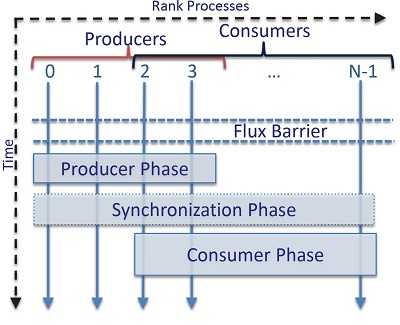
\includegraphics[scale=0.45]{kaptester}
%  \caption{Main phases of KAP tester}
%  \label{fig:kap}
%\end{figure}
KAP models KVS access patterns through various interactions
between KVS writers and readers. Writers are called producers;
readers consumers.
In essence, KAP allows a configurable number of producers
to write key-value objects into our KVS 
and a configurable number of consumers to read these
objects after ensuring the consistent KVS state.

In addition to producer and/or consumer counts,
KAP provides a range of parameters that can affect performance.
Among them include the value size (of key-value objects),
the number of objects to put,
the number of objects to get, objects access 
patterns (through different striding), and
synchronization primitives used for consistency.
KAP consists of four phases: setup, producer, synchronization 
and consumer phases. 
During the setup phase, tester processes are launched 
into a set of nodes in which a CMB session had been established.
They are assigned ranks such that consecutive rank
processes are distributed to consecutive nodes.
The rank processes determine their roles based
on the command line arguments and issue a
\flux\ collective barrier to begin to play their roles
simultaneously.

Next, each producer calls the specified number of
{\tt kvs\_put}s of an object of the specified value size.
For each call, the producers use unique keys, but
the values can be configured to be either unique
or redundant.
Once this is done, all of the producers and consumers
enter the synchronization phase in which they 
participate in a consistency protocol. They use
KVS synchronization primitives such as {\tt kvs\_fence}
and {\tt kvs\_wait\_version}.
Finally, during the consumer phase, consumers read
these key-value objects by calling {\tt kvs\_get}s.
KAP provides options to emulate various read access
patterns.

